%!TEX root = ../main.tex

\chapter{Related Work}

\label{Chapter2-related-work}

\section{Transactional Dataflow Systems}

Transactional dataflow systems are a class of distributed systems designed to handle large-scale data processing with transactional guarantees.
They provide a programming model that allows developers to write declarative, data-driven computations that automatically handle fault tolerance, scalability, and consistency.

Transactional dataflow SFaaS (Stateful Function-as-a-Service) systems are cloud-based systems that provide a serverless platform for processing large-scale data with transactional guarantees.
These systems allow users to write and deploy stateful individual functions or small pieces of code that are triggered in response to events, such as incoming data or scheduled tasks. They are build on top of dataflow systems because they provide fault tolerance, scalability and consistency out-of-the-box.

One of the most prominent transactional dataflow SFaaS system is Apache Flink's [\cite{apache-flink}] StateFun, the architecture of which is shown in figure \ref{fig:statefun-arch} (credits to [\cite{transactions-serverless-functions-leveraging-stateful-dataflows}]).

\begin{figure}[h]
    \centering
    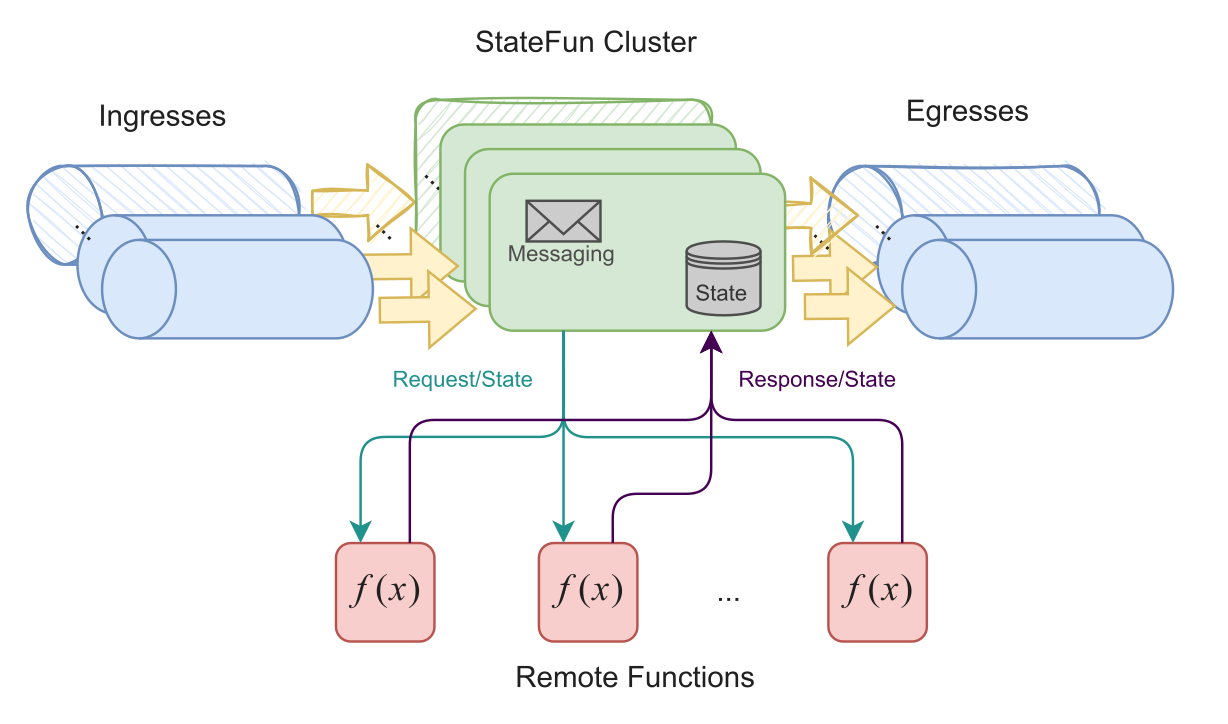
\includegraphics[width=0.8\textwidth]{statefun-arch.png}
    \caption{Architecture of Apache StateFun}
    \label{fig:statefun-arch}
\end{figure}

Remote functions are executed in the nodes of the StateFun cluster, and each node saves its state into an embedded key-value store, as the state can be modelled effectively by a collection of key-value pairs.
In relation to the current work, this is the model architecture for which we will optimize our key-value stores. More concretely, we assume that the key-value stores are to be used as embedded key-value stores in a similar cluster, and that there is some reliable remote storage in the cloud to store our snapshots.

\section{Key-value stores}

A key-value store is a type of database that uses a simple key-value data model to store data.
In a key-value store, data is represented as a collection of key-value pairs, where each key is a unique identifier that is associated with a corresponding value.

Key-value stores are designed for efficient and fast access to data, making them suitable for use cases where high performance and low latency are critical.

There are various types of key-value stores, each of which is optimized for specific use cases and applications. A fundamental factor that determines the properties of a key-value store is its backend, i.e. the data structures that power it. The main backends for key-value stores are B-Trees, LSM-Trees, and on-disk hash-tables if they store their data on disk, or other tree-based or hash-based data structures if they store their data in memory. Of course, there are also hybrids that combine other types.

\subsection{Types of key-value store backends}

\subsubsection{B-Trees}
% TODO - argue why you selected these databases, LSMT paper shits on B-trees so use that info from there

[TODO placeholder]
A B-tree is a data structure used in computer science to store and organize data in a sorted manner, allowing for efficient search, insertion, and deletion operations. It is a balanced tree structure, meaning that the height of the tree is kept relatively low compared to the number of elements it contains, which in turn ensures fast access and modification times.

The B-tree consists of nodes, each containing a number of keys and pointers to child nodes. The keys are sorted in ascending order within each node, and the pointers are used to traverse the tree and locate the desired key or node. The number of keys and pointers in each node is fixed, and typically determined by the size of a disk block or page.

B-trees are commonly used in database systems, file systems, and other applications that require fast and efficient access to large amounts of data stored on disk or in memory.

\subsubsection{LSM-Trees}

[TODO placeholder]
LSM-Trees are analyzed more in Chapter \ref{Chapter3-implementation}.

\subsubsection{Fractal Trees}

[TODO placeholder]

Fractal Trees are a type of indexing data structure that are designed to provide high performance and scalability in multi-core environments. They were first introduced in 2006 as an alternative to B-trees and LSM-trees.

The key idea behind Fractal Trees is to split the index into a set of smaller indexes, each of which is optimized for a specific data access pattern. This allows the system to scale horizontally across multiple cores and nodes, while also providing high performance for a wide range of workloads.

In a Fractal Tree, the index is partitioned into a set of subtrees, each of which is a complete and self-contained index. Each subtree is further divided into a set of smaller subtrees, with each level of the index optimized for a specific access pattern. This allows the system to optimize access to the data based on the specific needs of the application, providing high performance and scalability.

% One of the key benefits of Fractal Trees is that they can be used to provide high performance and scalability for a wide range of data access patterns, including read-heavy, write-heavy, and mixed workloads. They can also be used to provide high performance for a wide range of data sizes, from small to very large datasets.

% Fractal Trees have been used in a number of applications, including databases, file systems, and distributed storage systems. They are particularly well-suited for applications that require high performance and scalability in multi-core environments, such as cloud computing and big data analytics.

\subsubsection{On-disk hash-tables}

% Note, instead of B-trees there are also on disk hash-tables, like gdbm.

\subsubsection{In-memory key-value stores}

% \begin{enumerate}
%     \item LevelDB: A popular open-source key-value store that is optimized for read-heavy workloads and has a small memory footprint.
%     \item RocksDB: A fork of LevelDB that is designed to handle a wider range of workloads, including write-heavy ones.
%     \item LMDB: A high-performance, memory-mapped key-value store that supports multi-threading and transactions.
%     \item Cassandra: A distributed key-value store that is optimized for write-heavy workloads and provides tunable consistency levels.
%     \item Riak: A distributed key-value store that is designed for high availability and fault-tolerance and supports both eventual and strong consistency.
%     \item Berkeley DB: A mature and battle-tested embedded key-value store that supports transactions, replication, and high availability.
%     \item Kyoto Cabinet: An efficient and lightweight key-value store that is designed for high-speed data storage and retrieval.
%     \item Redis: A popular in-memory key-value store that also provides disk-based persistence, making it suitable for large datasets that cannot fit in memory.
% \end{enumerate}

\subsubsection{Hybrids}

% faster

\subsection{Key-value stores in dataflow systems}

% "In support of workload-aware streaming state management" for comparisons

\section{Incremental Snapshots}

% Merkle trees for synchronization?

% Differential Synchronization by neil fraser

% Lightweight Asynchronous Snapshots for Distributed Dataflows
% state management in apache flink: cite the paper with this name (section 4.2)
%% **** state management in apache flink section 4.2!!

% JSON crdt? and crdt paper "A comprehensive study of convergent and commutative replicated data types"

% see the intensive data book, explain write amplification.
% update: i won't explain it here, i will do it chap3 where it appears.